\section*{Unmanned Aerial System (UAS)}
In some cases it is necessary to talk about our system as a whole, such that we use it further. The UAS is composed of the following:
\begin{itemize}
	\item Drone
	\item Basestation
	\item Communications
	\item Survey camera
\end{itemize}

\begin{figure}[h!]\label{fig:uas}
	\centering
	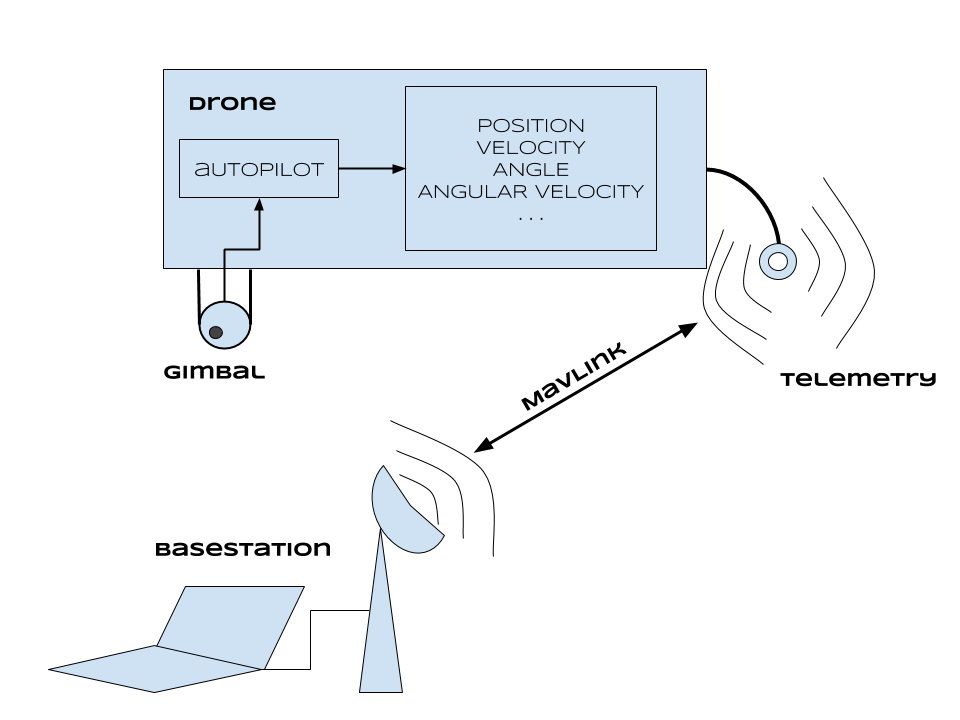
\includegraphics[width=0.7\textwidth]{figures/uas.png}
	\caption{Unmanned Aerial System Overview}
\end{figure}

\section*{Technical Scenario}
As mentioned before we need to assure the maximum distance of communication possible between the basestation and the drone at a certain working frequency:

\begin{equation*}\label{eq:tech_parameters1} 
 	\begin{cases}
 		d_{max} = 50 km	\\
 		f = 2.4 GHz
 	\end{cases}
\end{equation*}

\section*{Antenna Overview}
The antennas used for the basestation and the drone are different by means of weight and size. The preference of using them is based on the application at hand, thus for:
\begin{itemize}
	\item Basestation - Parabolic (grid) directional antenna 
	\item Drone - Patch directional antenna
\end{itemize}

A parabolic antenna in an antenna that uses a parabolic reflector and a curved surface to direct the radio waves and its main advantage is that it has a high directivity. This type of antennas are able to produce the narrowest beam widths which allow them to have some of the highest gains.

Parabolic antennas, due to their high gain, are intensively used for carry telephone and television signals between nearby cities. In our specific case, it’s possible to use this property to receive the information provided by the thermal camera through the UAS.

Patch antenna, which is the original type of microstrip, is a low profile antenna that can be mounted on a flat surface and it consists in a rectangular sheet of metal. These antennas are very useful because they are very thin and their directivity varies from 5 to 7 dB.

\begin{table}[h!]
\centering
	\begin{tabular}{|c||c|c|}
		\hline
		Parameter & Basestation & Drone\\ \hline\hline
		Type & Parabolic & Patch\\ \hline
		Polarization & Linear & Linear\\ \hline
		Frequency [GHz] & $2.4$ & $2.4$\\ \hline
		Gain [dB] & $24$ & $14$\\ \hline
		HPBW/$H(^{\circ})$ & $14$ & $45$\\ \hline
		HPBW/$V(^{\circ})$ & $10$ & $45$\\ \hline
	\end{tabular}
	\caption{Table of antennas parameters}
	\label{table:1}
\end{table}

\section*{Calculus of Radio Communication Parameters}

Computing signal wavelength ($\lambda$) for the working frequency stated above:
\begin{equation*}\label{eq:tech_parameters3}
	\lambda = \frac{c}{f} = \frac{3\cdot 10^{8}}{2.4\cdot 10^{9}} 
	        = 0.125 \text{m}
\end{equation*}

Computing the path loss for a distance of 50 kilometers and the signal wavelength:
\begin{equation*}\label{eq:tech_parameters4}
	L = 20lg\left (\frac{4\pi d_{max}}{\lambda} \right)
	  = 20lg\left (\frac{4\pi \cdot 50}{0.125\cdot 10^{-3}} \right)
	  = 134 \text{dB} 
\end{equation*}


Computing the output power of the transmitting antenna of 1 Watt:
\begin{equation*}\label{eq:tech_parameters5}
	P_{TX} = 10lg\left (\frac{1}{10^{-3}} \right)  
	       = 30 \text{dBm}
\end{equation*}


A simplified link budget omitting some losses of the UAS:
\begin{equation*}\label{eq:tech_parameters6}
	P_{RX} = P_{TX} + G_{TX} + G_{RX} - L  
	       = 30 + 24 + 14 - 134 = -126 \text{dBm}
\end{equation*}

